\chapter{Methodology}

\section{Data selection: Lightly supervised approach}
Despite of the high development in automatic speech recognition, there exist many challenges. One of the main challenge of speech recognition is to reduce development cost when adapting the speech recognition to other task or creating a new speech recognition for a new language. The biggest development cost is to transcribe the audio data with their exact corresponding transcriptions. To generate a "good" speech recognition, one needs a massive number of training audio and their exact transcriptions. However, transcribing audio is labor intensive and time consuming too. There are unlimited supply of audio data in the internet, television, radio, and other sources. Nonetheless, they usually have a few or even no accurate transcription at all.  Some television broadcasts have corresponding closed captions.  Closed caption means that the transcription is close, but not exactly the same as what the audio says. Even, the closed captions are often badly time-aligned with the audio.

By utilizing these audio data with the corresponding closed captions, we hope to produce a high performance speech recognizer with less supervision. The main idea is to use the automatic speech recognizer to transcribe audio data which will automatically generate transcriptions, which later be used as training data \cite{lightlySupervised}. The steps are as following. Firstly, we train a bootstrap acoustic model trained on a small manually annotated data. Then, recognize the data with closed captions by using the bootstrap model. We compare the decoding result from the bootstrap model with the closed captions and remove the words which do not agree. Finally, we can train a new acoustic model from the filtering.

The idea of using untranscribed audio data has been explored before(Zavaliagkos and Colthurst in 1998 \cite{Zavaliagkos1998UtilizingUT} and Kemp \& Waibel \cite{Kemp_unsupervisedtraining}), which is called as unsupervised acoustic model training. They utilized small amount of audio data without transcription to train acoustic models. The drawback of their experiments is not using massive volume of training data which is essential to train an acoustic model.

Lightly supervised approach was proposed in 2002 by Lamel et al \cite{lightlySupervised}. 
In general, the lightly supervised approach operates as following:
\begin{enumerate}
\item Train an acoustic model on a small amount of manually annotated data. 
\item Recognize(or automatically transcribe) a massive amount of data.
\item Align the automatic transcriptions with the closed captions. Some transcriptions and closed captions might disagree. We can remove or correct these segments.
\item Retrain a new acoustic model using the data which we selected in the previous step. 
\item Reiterate from step 2.
\end{enumerate}
These steps can be iterated several times as long as the error rate is decreasing. This method uses the idea of training acoustic model in less supervised manner because the training dataset(closed captions) is not the real detailed transcription. 

Using closed caption as training data reduces effort in manual transcription.Detailed transcription process usually takes 20-40 times manual effort compare to live closed captioning. Closed caption is usually produced in real time and less costly compare to the detailed transcription. In addition, the manual transcription is possible to have error \cite{Barras2001}. Additionally, some TV broadcasts, such as: CNN headline news, ABC world news tonight, BBC, already have closed captions which can be used as a training dataset. Nevertheless, some problems exist when using the data with closed captions as training dataset. However, training using  the closed captions faces several disadvantages compared to the real transcriptions: indication of non speech event, such as: coughing, speaker turn, acoustic conditions: background noise and music. Furthermore, some sentences might be paraphrased, deleted, and changed in word order. 

In addition to the closed captions, we can use additional data to build a language model. Other kinds of text are available in internet, such as: news, blog, and closed captions from TV broadcast. However, these data might be less related with the audio data. Some additional sources may be not contemporaneous with the data. Thus, it provides less supervision. We can interpolate these data with the closed captions to build a more general language model.

Despite the fact that closed captions are not accurate, it has been proven that closed captions provides enough supervision in building automatic speech recognition systems \cite{lightlySupervised}. Lamel found that an increase in training data improves accuracy even tough it will increase the model size. Additionally, filter closed captions for the next iteration training set in the lightly supervised technique improves the accuracy slightly. The language model built from closed captions also effectively provides enough supervision in building the ASR. Therefore, lightly supervised technique is our main inspiration to do data selection in this internship.

\section{State-of-the-art data selection}
Some researches have been conducted to investigate the lightly supervised approach to select data in the speech recognition problem\cite{lightlySupervised,Lecouteux06imperfecttranscript,Chan,Mathias,Stolcke00anefficient}. The state-of-the-art data selection was proposed by  Lanchantin et al from Cambridge university\cite{Lanchantin2016}. Before talking about the state-of-the-art, it is better to discuss some previous related works first.

Lamel et al proposed the lightly supervised approach which harnessed the closed caption as supervision to build a robust speech recognizer\cite{lightlySupervised}. In their experiment, they used a bootstrap acoustic model and biased language model to recognize the audio where the decoding result is compared with the closed caption. Then, the words which do not agree will be removed from training dataset. The new training dataset is utilized to train a  new acoustic model. This filtering(removing not-agree words) is called closed caption filtering.

Chan and Woodland explored another way in filtering bad closed captions\cite{Chan}. They leveraged the confidence measure metric to remove the bad segments. When decoding acoustic inputs, an ASR produces word hypothesis and their corresponding confidence measure. The confidence measure value from each word in  each segment is averaged to produce one confidence value per segment. Finally, they determined a threshold confident value to filter out all potentiallly bad segments, where the confident value is lower than the threshold. Moreover, they also introduced to interpolate two different LMs created from two closed caption datasets and merge them into one single LM. This single LM is used as light supervision when decoding acoustic input together with the acoustic model and the lexicon.

Matias et al applied lightly supervised approach on medical conversation data \cite{Mathias}. There are unlimited supplies of medical speech; however, only informal medical reports are available. The medical reports are not the same as what the physicians said in the audio records. This problem matches perfectly with the lightly supervised approach. They explored frame level filtering in place of word level or segment level filtering. Basically, they forced align and compared the decoding results with the closed captions and mark words which are insertion, deletion, and substitution. All corresponding frames which are associated with those marked words are removed or filtered out from training set to produce a new cleaner training set.

The state-of-the-art data selection was proposed by  Lanchantin et al from Cambridge university\cite{Lanchantin2016}. They used the lightly supervised approach applied on the multi genre broadcast(MGB) challenge. MGB challenge is a challenge to automatically transcribe TV broadcasts. The challenge only provided TV broadcast audio data and their corresponding closed captions. General TV broadcast data are usually recorded in highly diverse environment speech with background music, non speech event, and sound effect. In addition, some closed captions may be different compared to the real transcription due to deletion, insertion, substitution, and paraphrasing. These factors make the challenge interesting as well as complicated. 

Lanchantin et al proposed to tackle the problem inspired from the lightly supervised approach. The lightly supervised approach works as following \cite{Lanchantin2015}.
\begin{enumerate}
\item Trained an acoustic model by selecting a subset of 200 hours training set from the total 1600 hours training set. We called this as AM-v1 which is based on deep neural network.
\item AM-v1 recognized the entire training dataset(1600 hours) which resulted in the decoding result. Compare and force aligned the decoding result with the closed captions. By comparing each segment, they calculated phone matched error rate(PMER) and word  matched error rate(WMER) as well as average word duration.
\item By utilizing average word duration and phone matched error rate, they selected 700 hour of data(700hr-v1). The way to select the data is 
\begin{enumerate}
\item Reject segments which are not in the range of $0.165 \leq AWD \leq 0.66$
\item Sort segments based on PMER and select the top segments until reaching 700 hours set. The threshold for this iteration is $40\%$. This new selected training data is called 700-v1.
\end{enumerate}
\item Retrain a new acoustic model using the 700-v1. Repeat step 2-4 to create 700-v2, 700-v3 until the data selection algorithm converges. 
\end{enumerate}

In every iteration, the language model which they utilized are the same. MGB provides closed captions for each audio and additional text consisting 10 million and 640 million words respectively. From these texts, two language models were built and interpolated into one language model. Furthermore, the merged language model was pruned by $10^{-9}$ to expedite the decoding process.

A question remains to be asked: when to stop the iteration(the algorithm converges)? The MGB challenge provides a development set which comprises of audio data and their manually transcribed transcriptions. These transcriptions are exactly what people said in the audio with correct time stamp. By recognizing the development set with the ASR system which they built in each iteration, they calculated word error rate(WER). If the WER decreases in the next iteration, continue the iteration. Otherwise, stop the iteration.






\section{Data}
Before talking about the methodology, it is better to talk about the dataset. We have the following dataset:
\begin{enumerate}
\item Training set has audio data with their corresponding closed captions.
\item Test set has audio data and their corresponding manual transcriptions. These manual transcriptions are the same as what people said in the audio.
\item Additional text corpus which is utilized for building language model. This additional corpus is different than the closed captions in training set. 
\end{enumerate}




\section{Language model}



\section{Acoustic model}

\section{Data selection}

%\textbf{Insert time and perpelexity here.}

\section{Baseline model}

\subsection{Acoustic model AM.200 and Language Model Version 1 (LM.200.1e-9)}
\label{amv0s1}


Calculating PMER and WMER for each segment by utilizing AM.200 and LM.200.1e-9:
\begin{enumerate}
\item GMM(GMM.200): GMM is trained by using the 200 hours data
\item TDNN(TDNN.200): the result of GMM training(GMM.200) is utilized to build a TDNN(time delay neural network). 
\item TDNN graph creation \\
The language model used is the LM.200.1e-9 and  the acoustic model is  TDNN.200; furthermore, the dictionary used(Lexicon.200) is the modification of the library provided by MGB(Lexicon.MGB). Words in Lexicon.MGB which do not exist in word.200 are removed from Lexicon.200.
%\item TDNN development set recognition \\
%The development set is files from dev.short, which contains 8 hours of audio. The development set is recognized by leveraging the graph created in the previous step.
\item TDNN 200 hours of training data recognition \\
We need to recognize 200 hours data to calculate PMER, WMER, and AWD. This data will be used for data selection of the next iteration.
\item Sclite score PMER and WMER \\
Use the lattice and graph(produced at step 5 and 3 respectively) to calculate overall PMER and WMER. However, the decoding program does not provide PMER, WMER, and AWD for each segment. Fortunately, the program generates prf file which contains number of correction, insertion, deletion, and substitution for each segment. Two prf files exist after decoding:(ctm\_words.filt.filt.prf contains word match error rate and ctm\_phones.filt.filt.prf contains phone match error rate). From there, we are able to calculate  PMER, WMER, and AWD of each segments.  For the development set, we only need to know the overall PER and WER. In contrast, training set recognition needs PMER, WMER, and AWD for each segment. 

\end{enumerate}


version AM0
% table
\begin{center}
\begin{tabular}{ | c | c | c | c |  c |  }
\hline
\textbf{No.} & \textbf{Description} & \textbf{Result} & \textbf{execution time} & \textbf{extra info} \\ \hline \hline
1 & GMM.100  &  & 3h 30m & 20 hosts \\  \hline
%/talc2/multispeech/calcul/users/jkarsten/mgb/recipe/tools/baseline/baseline1_backup/gmm
%1.1 & GMM decoding & 57.2\% WER  & 3h 36m 47s & 20 hosts, 4 cores \\  \hline \hline
%2 & AM.200 training. &  & 38h 30m 31s & 3 nodes \\  

2 & TDNN.100 training: & & 17h 7m & 3 GPU hosts \\ 
 & LM.200.1e-9,  GMM.100, Lexicon.200 &  & & \\ \hline
 %/talc2/multispeech/calcul/users/jkarsten/mgb/recipe/tools/baseline/baseline1_backup/tdnn
 
3 & Create a graph from TDNN.200,  &  & 6m & 1 host \\  
 & LM.200.1e-9, Lexicon.200  & & & \\ \hline
%/talc2/multispeech/calcul/users/jkarsten/mgb/recipe/tools/modifASR/tdnn_s1/graph_creation_from_arpaLM

4 & Create a graph from TDNN.200,  &   & 4h 49m & 1 host \\  
 & LM.7weeks+subtitles.1e-9, Lexicon.200  & & & \\ \hline

%4 & AM.200 recognized dev.short &  & 2h 58m 58s   & 20 hosts  \\  \hline
5 & TDNN.100 recognized train.200 &  & 16h 6m & 20 hosts \\  \hline 
 %/talc2/multispeech/calcul/users/jkarsten/mgb/recipe/tools/modifASR/tdnn_s1/recognition_with_scoring/decode_res_train_200_fst+merall_mgb2015.wordList.4gm.kn.arpa.gz.1e-9.arpa_4thr

6 & TDNN.100 \& LM.7weeks+subtitles.1e-9 & WER 43.9\%   & 45m & 20 hosts \\  
&  recognized dev.short & PER 35.8\% & & \\ \hline
%5 & Calculate Overall PMER & 24.8 \% PMER   & 5h 5m 51s & 1 host \\  \
 %& and WMER of train.200  & 32.4 \% WMER & & \\ \hline
%5.1 &  Calculate PMER and WMER & & 20m 22s & 1 host \\  
 %&  per segment of step 6 & & &  \\  \hline
%/talc2/multispeech/calcul/users/jkarsten/mgb/recipe/tools/modifASR/tdnn_s1/sclite_score_pmer_and_wmer
% /talc2/multispeech/calcul/users/jkarsten/mgb/recipe/tools/modifASR/tdnn_s1/calculate_pmer_wmer_per_segments

%6 & Calculate PER  &  32.5 \% PER  & 1h 10m 57s   & 1 host \\  \
% & PMER, WMER calculation  &   48.7\% WER   & & \\ \hline
\end{tabular}
\end{center}


%%%%%%%%%%%%%%%%%%%%%%%%%%%%%%%%%%%%%%%%
% table
version AM1
\begin{center}
\begin{tabular}{ | c | c | c | c |  c |  }
\hline
\textbf{No.} & \textbf{Description} & \textbf{Result} & \textbf{execution time} & \textbf{extra info} \\ \hline \hline
1 & GMM.100  &  & 4h 7m & 20 hosts \\  \hline

2 & TDNN.100 training: & & 20h 1m & 3 GPU hosts \\ 
 & LM.200.1e-9,  GMM.100, Lexicon.200 &  & & \\ \hline
 
3 & Create a graph from TDNN.200,  &  & 5m & 1 host \\  
 & LM.200.1e-9, Lexicon.200  & & & \\ \hline
 
4 & Create a graph from TDNN.200,  &   & 3h 7m & 1 host \\  
 & LM.7weeks+subtitles.1e-9, Lexicon.200  & & & \\ \hline

5 & TDNN.100 recognized train.200 &  & 14h 18m & 20 hosts \\  \hline 

6 & TDNN.100 \& LM.7weeks+subtitles.1e-9 & WER 41.2\%   & 46m & 20 hosts \\  
&  recognized dev.short & PER 33.8\% & & \\ \hline
\end{tabular}
\end{center}

%%%%%%%%%%%%%%%%%%%%%%%%%%%%%%%%%%%%%%%%
version AM2
\begin{center}
\begin{tabular}{ | c | c | c | c |  c |  }
\hline
\textbf{No.} & \textbf{Description} & \textbf{Result} & \textbf{execution time} & \textbf{extra info} \\ \hline \hline
1 & GMM.100  &  & 3h 3m & 20 hosts \\  \hline

2 & TDNN.100 training: & & 23h 58m & 3 GPU hosts \\ 
 & LM.200.1e-9,  GMM.100, Lexicon.200 &  & & \\ \hline
 
3 & Create a graph from TDNN.200,  &  & 5m & 1 host \\  
 & LM.200.1e-9, Lexicon.200  & & & \\ \hline
 
4 & Create a graph from TDNN.200,  &   & 3h 13m & 1 host \\  
 & LM.7weeks+subtitles.1e-9, Lexicon.200  & & & \\ \hline

5 & TDNN.100 recognized train.200 &  & 15h 51m & 20 hosts \\  \hline 

6 & TDNN.100 \& LM.7weeks+subtitles.1e-9 & WER 40.5\%   & 36m & 20 hosts \\  
&  recognized dev.short & PER 33.3\% & & \\ \hline
\end{tabular}
\end{center}


%%%%%%%%%%%%%%%%%%%%%%%%%%%%%%%%%%%%%%%%
version AM2
\begin{center}
\begin{tabular}{ | c | c | c | c |  c |  }
\hline
\textbf{No.} & \textbf{Description} & \textbf{Result} & \textbf{execution time} & \textbf{extra info} \\ \hline \hline
1 & GMM.100  &  & 3h 3m & 20 hosts \\  \hline

2 & TDNN.100 training: & & 25h 27m & 3 GPU hosts \\ 
 & LM.200.1e-9,  GMM.100, Lexicon.200 &  & & \\ \hline
 
3 & Create a graph from TDNN.200,  &  & 7m & 1 host \\  
 & LM.200.1e-9, Lexicon.200  & & & \\ \hline
 
4 & Create a graph from TDNN.200,  &   & 4h 49m & 1 host \\  
 & LM.7weeks+subtitles.1e-9, Lexicon.200  & & & \\ \hline

5 & Create a graph from TDNN.200,  &   & 2h 1m each genre & 1 host \\  
 & LM.genres.1e-9, Lexicon.200  & & & \\ \hline

6 & TDNN.100 recognized train.200 &  & 15h 52m & 20 hosts \\  \hline 

7 & TDNN.100 \& LM.7weeks+subtitles.1e-9 & WER 40.5\%   & 38m & 20 hosts \\  
&  recognized dev.short & PER 33.3\% & & \\ \hline
\end{tabular}
\end{center}



%\subsection{Acoustic model AM.200 and Language Model LM.7weeks+subtitles.limited.1e-9}
% table
%\begin{center}
%\begin{tabular}{ | c | c | c | c |  c |  }
%\hline
%\textbf{No.} & \textbf{Description} & \textbf{Result} & \textbf{execution time} & \textbf{extra info} \\ \hline \hline
%3 & Create a graph from TDNN.200,  &  & 3h 12m 25s & 1 host \\   
% & LM.7weeks+subtitles.limited.1e-9,   & & & \\ 
% & Lexicon.7weeks+subtitles & & & \\ \hline
 %/talc2/multispeech/calcul/users/jkarsten/mgb/recipe/tools/modifASR/tdnn_s2/graph_creation_from_arpaLM


%4 & TDNN.200 &  & 1h 10m 59s & 20 hosts \\  
% & recognized dev.short & & & \\ \hline
% /talc2/multispeech/calcul/users/jkarsten/mgb/recipe/tools/modifASR/tdnn_s2/recognition_human/recognition_with_scoring_human


 %5 & TDNN.200 recognized &  & 10h 9m 35s & 20 hosts \\  
 %& train.200 & & & \\ \hline  
 %/talc2/multispeech/calcul/users/jkarsten/mgb/recipe/tools/modifASR/tdnn_s2/recognition_with_scoring
 
% 6 & TDNN AM.200 dev short & 31.8\% PER  & 4h 58m 26s & 1 hosts \\  
% & PMER, WMER calculation & 49.5\% WER & & \\ \hline
% 6.1 & TDNN AM-V0 train 200 & 26.4\% PMER & 4h 58m 26s & 1 hosts \\  
% & PMER, WMER calculation & 39.7\% WMER  & & \\ \hline
% 6.2 & Calculate PMER, WMER &  &  & 1 hosts \\  
 %& AWD per segment &  & & \\ \hline \hline
%\end{tabular}
%\end{center}


\subsection{Acoustic model(AM.200) and Language Model version 3(LM.genres)}


\subsection{Acoustic model AM.100-v1 and Language Model version 1 (LM.200.1e-9)}
% table
\subsubsection{100 hours selection(100-v1)}
How to select 100 hours subset of data for baseline model v1:
Section \ref{amv0s1}  calculates PMER, WMER, and AWD for each segments. Consequently, we can extract segments(of 200 hours transcriptions) which satisfy $0.165 \le AWD \le 0.66$. In the other word, the segments which does not satisfy are removed. Then, segments are sorted based on their PMER in ascending. We can deduce PMER threshold  and its total duration by sorting PMER as presented in the following table:  
\begin{center}
\label{pmerAM0s1}
\begin{tabular}{ | c | c | c | }
\hline
\textbf{PMER} & \textbf{Total duration} & \textbf{Percentage of total segment duration}  \\ \hline \hline
0.0 & 14.83 h & 10\% \\ \hline
5 & 29.66 h & 20\% \\ \hline
10 & 44.49 h & 30\% \\ \hline
16 & 59.32 h & 40\% \\ \hline
24 &  74.15 h & 50\% \\ \hline
33 & 88.98 h & 60\% \\ \hline
47 & 103.81 h & 70\% \\ \hline
82 & 118.64 h & 80\% \\ \hline
\end{tabular}
\end{center}


%PMER: 0.0; duration: 53389.43; percentage: 0.100003435255
%PMER: 0.05; duration: 106776.9; percentage: 0.200003199245
%PMER: 0.1; duration: 160166.65; percentage: 0.30000723389
%PMER: 0.16; duration: 213552.14; percentage: 0.400003289154
%PMER: 0.24; duration: 266939.76; percentage: 0.500003334108
%PMER: 0.33; duration: 320342.37; percentage: 0.600031456745
%PMER: 0.47; duration: 373713.84; percentage: 0.700001251227
%PMER: 0.82; duration: 427112.53; percentage: 0.800022031335

The Table \ref{pmerAM0s1} shows that 60\% of data has 33\% PMER with total duration of 88.98 hours of audio. From the table, we conclude that threshold 33 is selected as the threshold to select data for the next iteration.

\begin{center}
\label{wmerAM0s1}
\begin{tabular}{ | c | c | c | }
\hline
\textbf{WMER} & \textbf{Total duration} & \textbf{Percentage of total segment duration}  \\ \hline \hline
0.0 & 14.83 h & 10\% \\ \hline
8 & 29.66 h & 20\% \\ \hline
15 & 44.49 h & 30\% \\ \hline
23 & 59.32 h & 40\% \\ \hline
32 &  74.15 h & 50\% \\ \hline
43 & 88.98 h & 60\% \\ \hline
58 & 103.81 h & 70\% \\ \hline
98 & 118.64 h & 80\% \\ \hline
\end{tabular}
\end{center}

\subsubsection{Training Acoustic model AM.100-v1}



%\begin{center}
%\begin{tabular}{ | c | c | c | c |  c |  }
%\hline
%\textbf{No.} & \textbf{Description} & \textbf{Result} & \textbf{execution time} & \textbf{extra info} \\ \hline \hline
%1 & GMM.100-v1 &  & 3h 28m 43s & 20 hosts \\  \hline
%2 & TDNN.100-v1 &  & 26h 5m 3s & 3 hosts \\  \hline
%3 & GMM.100-v1\_decode &  & 2h 51m 4s & 20 hosts \\  \hline
%4 & TDNN.100-v1\_decode &  & 24h 30m 31s & 3 hosts \\  \hline
%\end{tabular}
%\end{center}


\subsection{The Second Acoustic model(AM.100-v2) and Language Model version 1 (LM.200.1e-9)}


%\begin{figure}
%\caption{Graph of PMER and WMER produced transcription AM-V0 and LM s1. The red line represents PMER, while the blue line represents WMER.}
%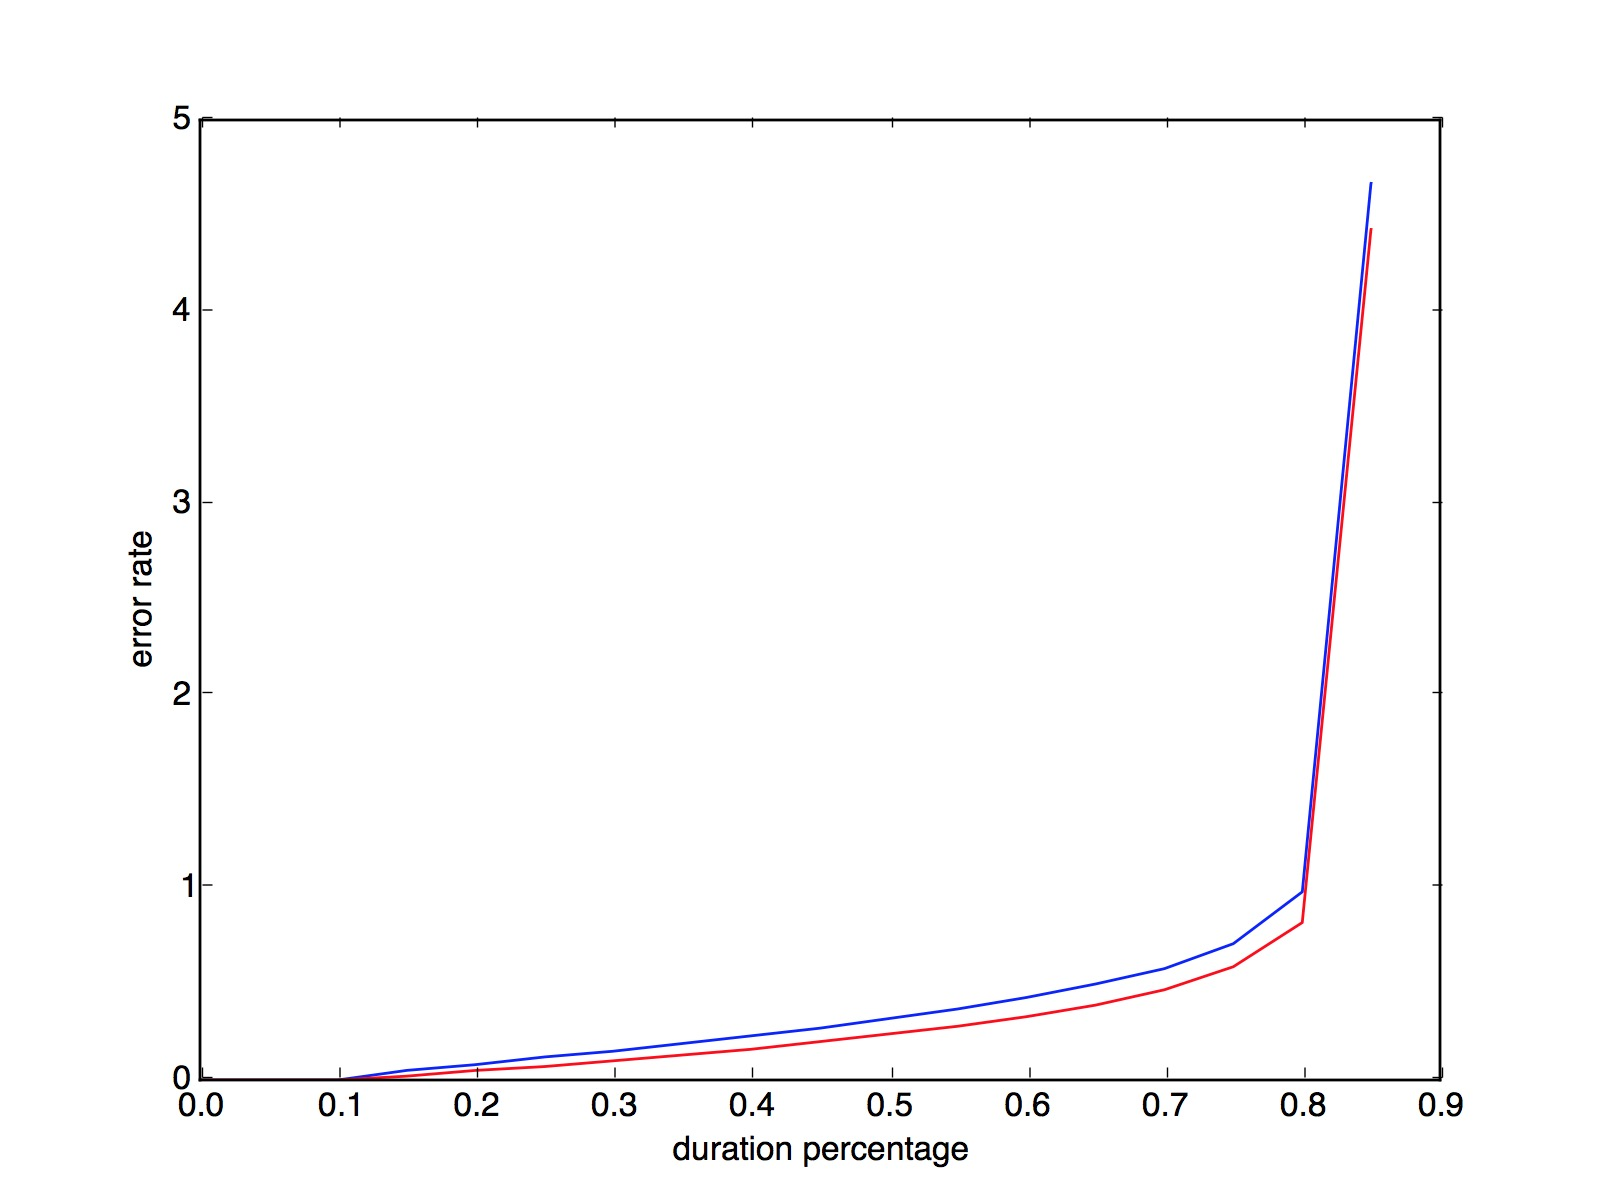
\includegraphics[scale=0.2]{wmerpmeram0s1} 
%\centering
%\end{figure}

%\begin{figure}
%\caption{Graph of PMER and WMER from transcription align, provided by MGB.}
%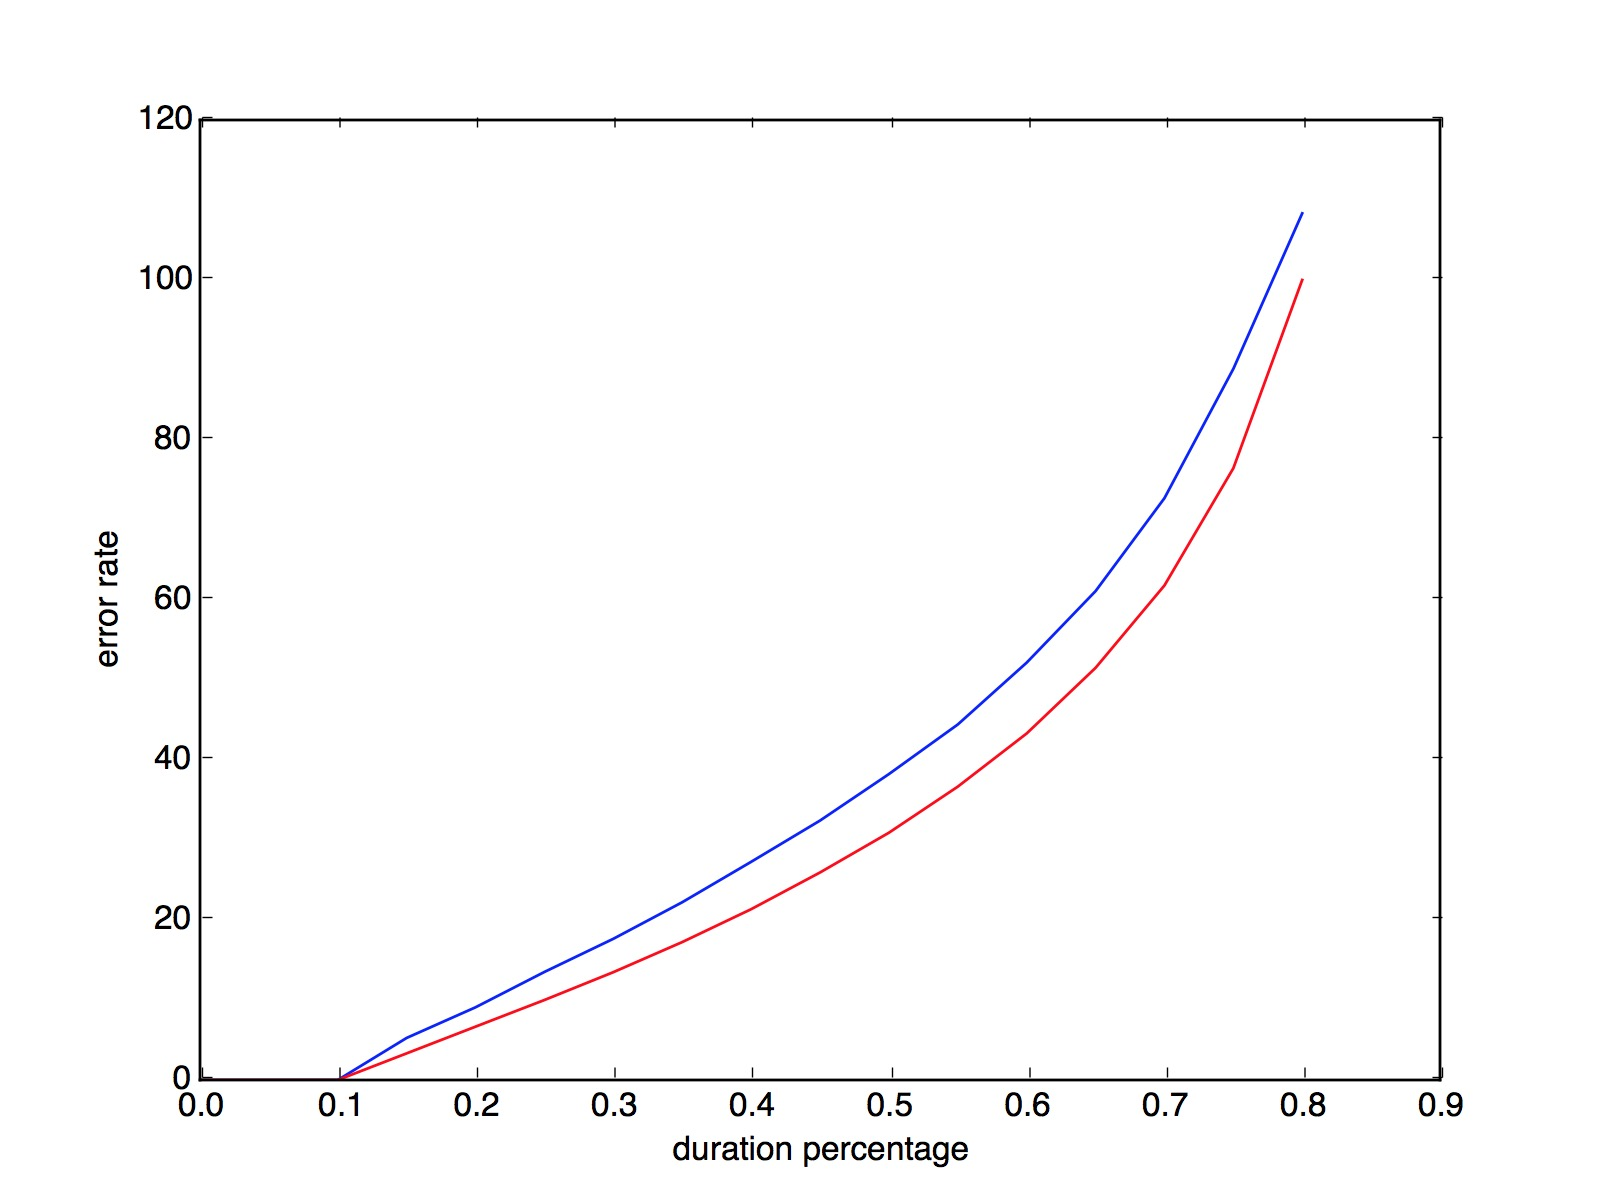
\includegraphics[scale=0.2]{wmerpmeram0align}
%\centering
%\end{figure}

%\subsubsection{Training acoustic model AM.100-v2}
%\begin{center}
%\begin{tabular}{ | c | c | c | c |  c |  }
%\hline
%\textbf{No.} & \textbf{Description} & \textbf{Result} & \textbf{execution time} & \textbf{extra info} \\ \hline \hline
%1 & GMM-V2\_decode &  & 2h 56m 41s & 20 hosts \\  \hline
%2 & TDNN-V2\_decode &  & 23h 52m 58s & 3 hosts \\  \hline
%\end{tabular}
%\end{center}


\section{Comparison}

Comparison between different speech recognizer:
\begin{center}
\label{wmerAM0s1}
\begin{tabular}{ | c | c | c |  c | c |  }
\hline
\textbf{No.} & \textbf{Acoustic model} & \textbf{Language Model}  &  \textbf{PER}  & \textbf{WER}  \\ \hline \hline
1 & TDNN.100  & LM.7weeks+subtitles.limited.1e-9 & 35.8  & 43.9 \\ 
& & Lexicon.7weeks+subtitles  & & \\ \hline


2 & TDNN.100-v1\_decode   & LM.7weeks+subtitles.limited.1e-9  & 34.3    & 42.3 \\
&  & Lexicon.7weeks+subtitles & & \\ \hline

3 & TDNN.100-v1   & LM.7weeks+subtitles.limited.1e-9  & 33.8   & 41.2 \\
&  & Lexicon.7weeks+subtitles & & \\ \hline


4 & TDNN.100-v2   & LM.7weeks+subtitles.limited.1e-9  & 33.3    & 40.5 \\
&  & Lexicon.7weeks+subtitles & & \\ \hline

5 & TDNN.100-v3   & LM.7weeks+subtitles.limited.1e-9  & 33.3    & 40.5 \\
&  & Lexicon.7weeks+subtitles & & \\ \hline
\end{tabular}
\end{center}


\begin{figure}
\caption{Average word duration}
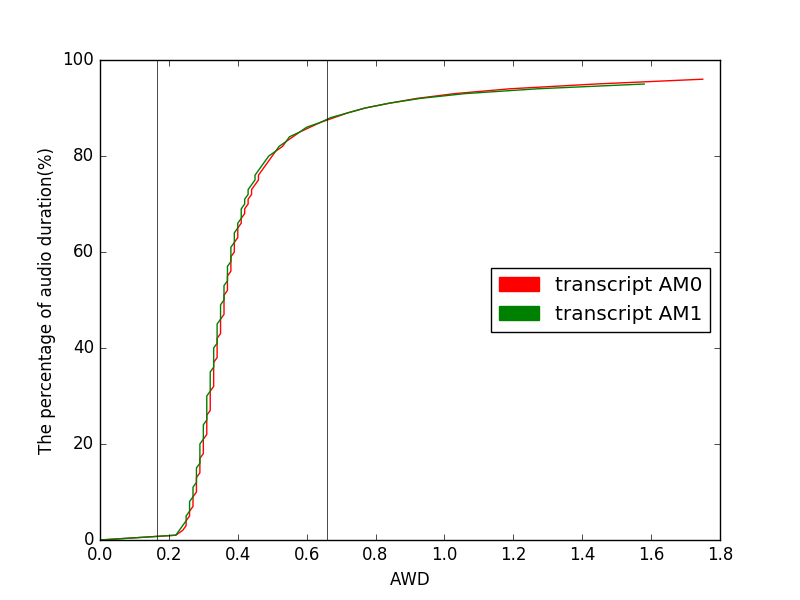
\includegraphics[scale=0.7]{awdLineChart}
\centering
\end{figure}

\begin{figure}
\caption{Phone match error rate}
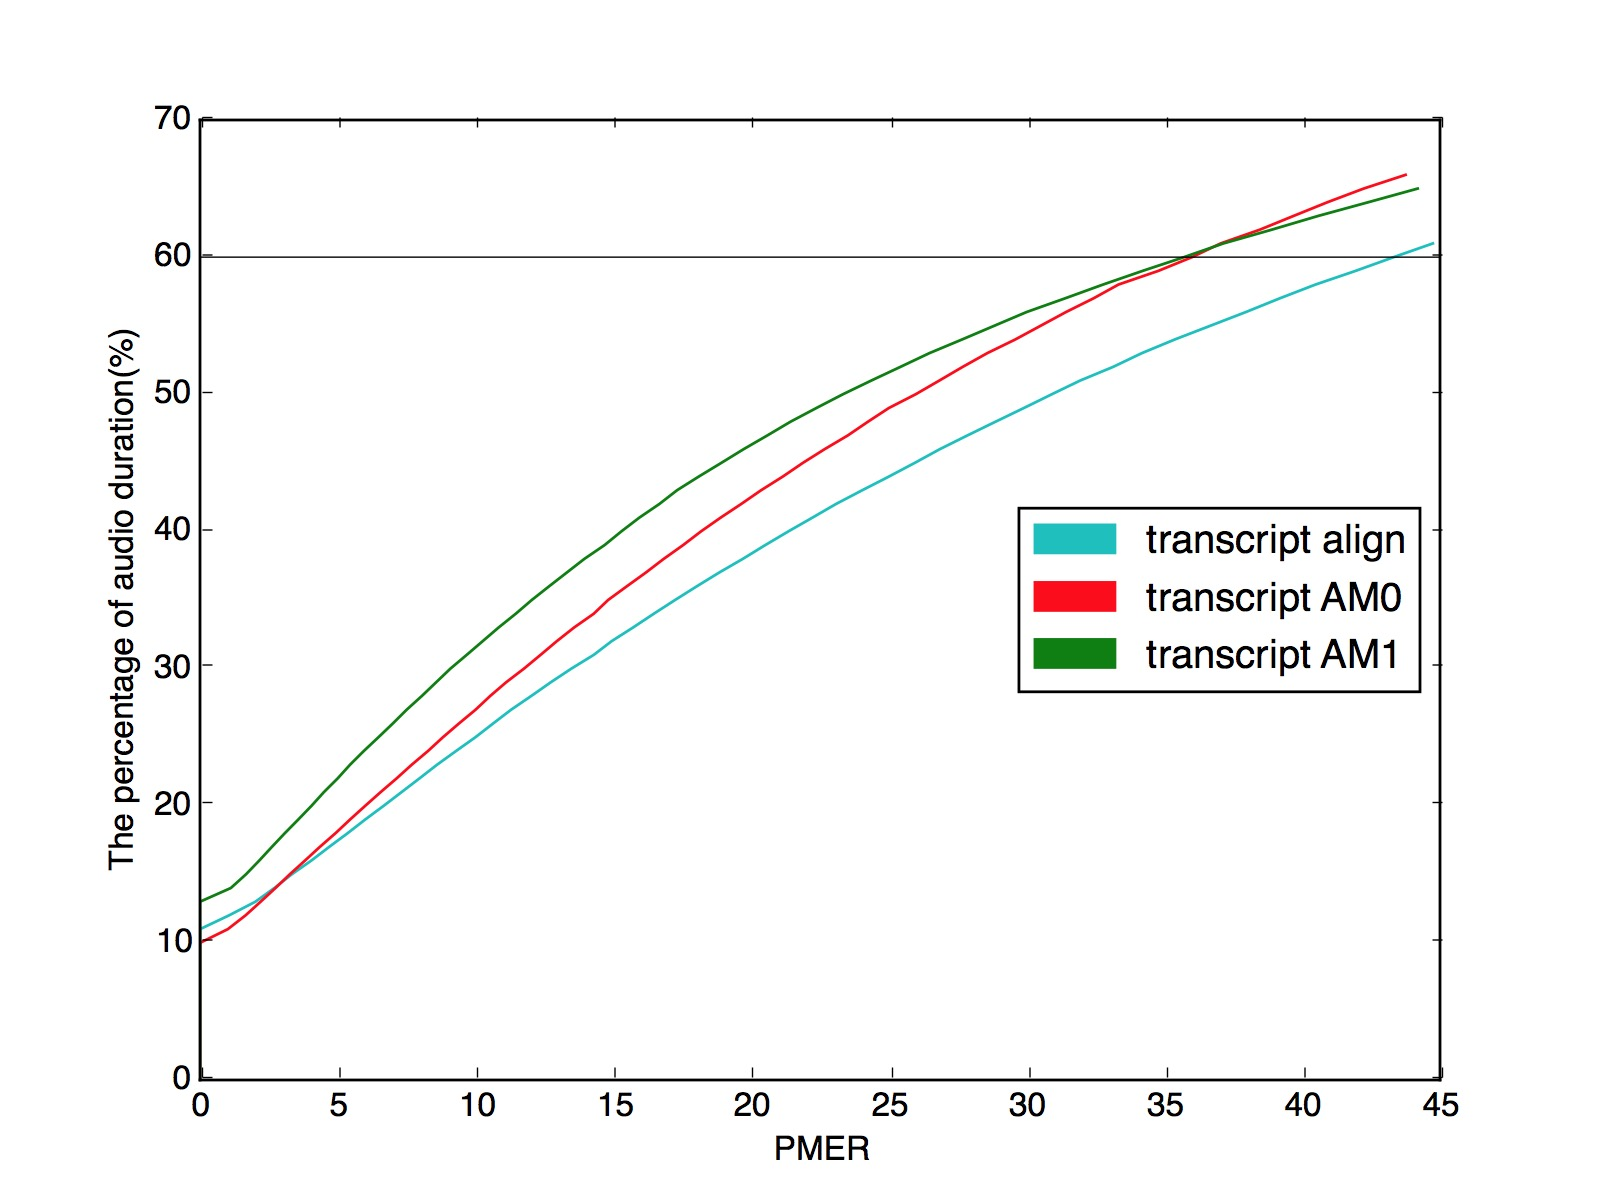
\includegraphics[scale=0.3]{pmerLineChart}
\centering
\end{figure}

\begin{figure}
\caption{Word match error rate}
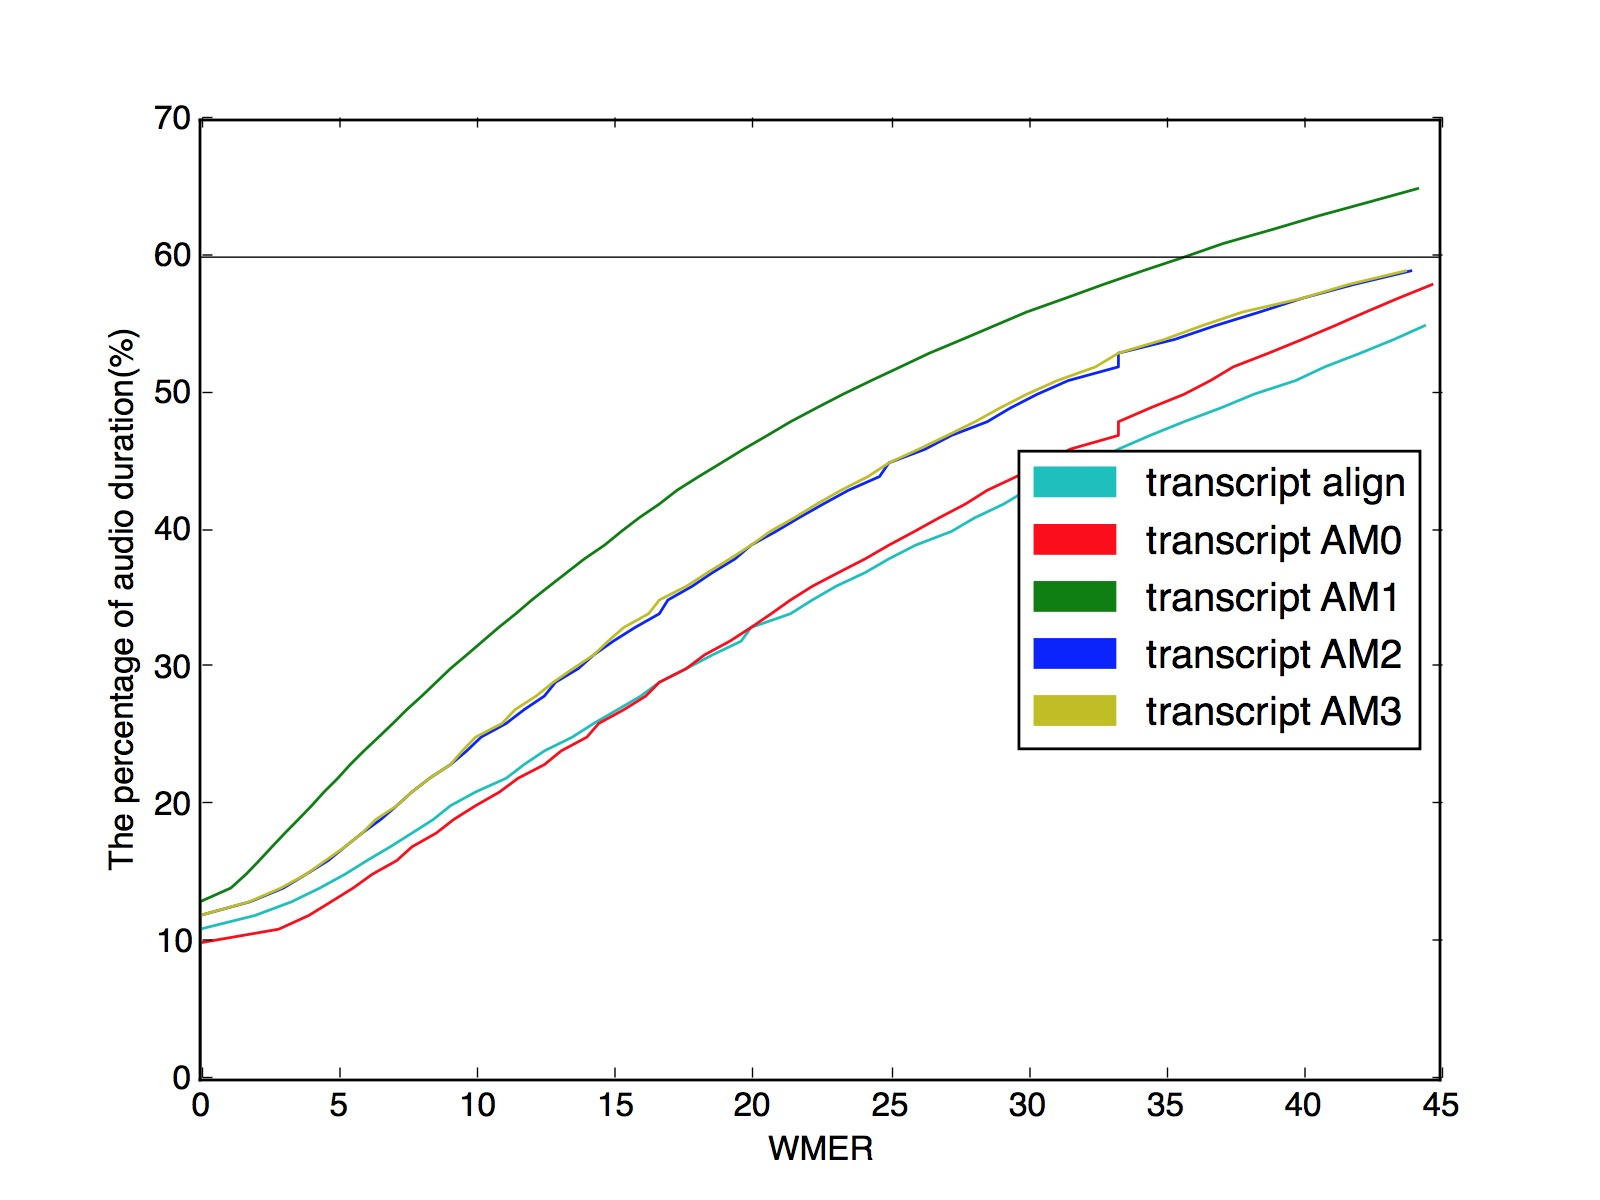
\includegraphics[scale=0.25]{wmerLineChart}
\centering
\end{figure}




%PER 32.2 | 9118 204786 | 75.0 10.0 15.0 7.2 32.2 82.7 | -1.058 | |
%WER 49.3 | 9118 64248 | 59.0 25.1 15.9 8.2 49.3 83.7 | -0.822 | |

%AM0_s1
%WMER
%[0, 0.05001182297101408, 0.1000055705823501, 0.15002999947778156, 0.20000377990423135, 0.250006911717846, 0.3000083202847346, 0.350008061797726, 0.4000080655439148, 0.45000218777410367, 0.5000070802963298, 0.5500076834326855, 0.6000113209817511, 0.6500022214898035, 0.7000031243212423, 0.7500004870045146, 0.8000498093227562, 0.8500152732106541]
%[0, 0.0, 0.0, 0.05, 0.08, 0.12, 0.15, 0.19, 0.23, 0.27, 0.32, 0.37, 0.43, 0.5, 0.58, 0.71, 0.98, 4.67]

%PMER
%[0, 0.05000255115439209, 0.10000343525488571, 0.15000458158857732, 0.20000319924500873, 0.2500218028172682, 0.3000072338900607, 0.3500012437345947, 0.4000032891535333, 0.45000364878763255, 0.5000033341077957, 0.5500060913025576, 0.6000314567451253, 0.6500026335705453, 0.700001251226977, 0.7500149847541436, 0.8000220313347739, 0.8500007005372576]
%[0, 0.0, 0.0, 0.02, 0.05, 0.07, 0.1, 0.13, 0.16, 0.2, 0.24, 0.28, 0.33, 0.39, 0.47, 0.59, 0.82, 4.43]

%Align
%WMER
%([0, 0.050002832118532126, 0.10000931677088468, 0.15000742869186362, 0.20000679558600154, 0.2500274408310134, 0.30000118379557716, 0.3500026485552931, 0.40000639849001596, 0.4500279240893308, 0.5000118004938804, 0.5500090133296115, 0.6000040159141051, 0.6500046752432919, 0.7000030681284111, 0.7500003184260248, 0.800006522114234], [0, 0.0, 0.0, 5.26, 9.09, 13.51, 17.65, 22.22, 27.27, 32.43, 38.24, 44.44, 52.17, 61.11, 72.73, 88.89, 108.33], 'b-'

%PMER
%[0, 0.05001950265750902, 0.10000225520549781, 0.15000134113549585, 0.20000690797165727, 0.25000294075800095, 0.30001437037921774, 0.35000064434442896, 0.40001250477732614, 0.45001977612927163, 0.5000107890229769, 0.5500005656744683, 0.60003347968693, 0.6500121301584764, 0.7000086499493287, 0.7500019667489803, 0.800000340903153], [0, 0.0, 0.0, 3.33, 6.67, 10.0, 13.48, 17.24, 21.35, 25.94, 30.91, 36.67, 43.32, 51.52, 61.82, 76.47, 100.0], 'r-'

